\section{Performance}

%This section needs material to be written.
%Figures to be prepared and included:
%\begin{itemize}
%\item{vertex time resolution, integrated and per paddle}
%\item{z difference CND/CVT, per paddle}
%\item{a plot showing the quality of energy calibration}
%\item{the plot of energy deposit versus beta, showing neutrons, photons, and background, from RGB data;}
%\item{neutron efficiency, possibly versus momentum, obtained from $ep\to en\pi^+$ events (RGA, low energy)}
%\end{itemize}
Data taken during the first CLAS12 experiments, on hydrogen and deuterium targets, and with various beam energies (6.6 and 10.6 GeV), were analyzed to verify the performances of the CND. 

The timing performances for the three layers of the CND are illustrated in Fig.~\ref{fig_performance_deltat_layers}, that shows the vertex time difference $v_t$ for selected negative tracks, integrated over all sectors. It is defined as
\begin{equation}\label{eq_vtp_definition}
v_t=t_{\rm{CND}}-t_{\rm{S}}-\frac{path}{c \cdot \beta}
\end{equation}
where $t_{\rm{S}}$ is the event start time determined by the FTOF, $path$ is the distance, computed by the CVT, travelled by the particle from the target to the CND impact point, and
\begin{equation}\label{eq_beta_definition}
\beta=\frac{p}{\sqrt{p^2+m^2}} .
\end{equation}
% e
The distribution of $v_t$ is centered at 0, and from its width, obtained with a Gaussian fit ($\sigma_{v_t}\simeq 243$ ps in average) one can deduce the average timing resolution for each PMT of the CND, convoluted with the CVT resolution, using the formula:
\begin{equation}\label{eq_resolution}
\sigma_t=\frac{\sqrt{\sigma_{v_t}^2-\sigma_{t_{S}}^2}}{\sqrt{2}}=157 ps, 
\end{equation}
assuming $\sigma_{t_{S}}=80$ ps \cite{ftofref}. This is compatible with the detector specifications (150 ps) and the result of the measurements in cosmic rays during the detector assembly phase \cite{Niccolai:2018qzm} (148 ps).

\begin{figure}[htb]  
\begin{center}
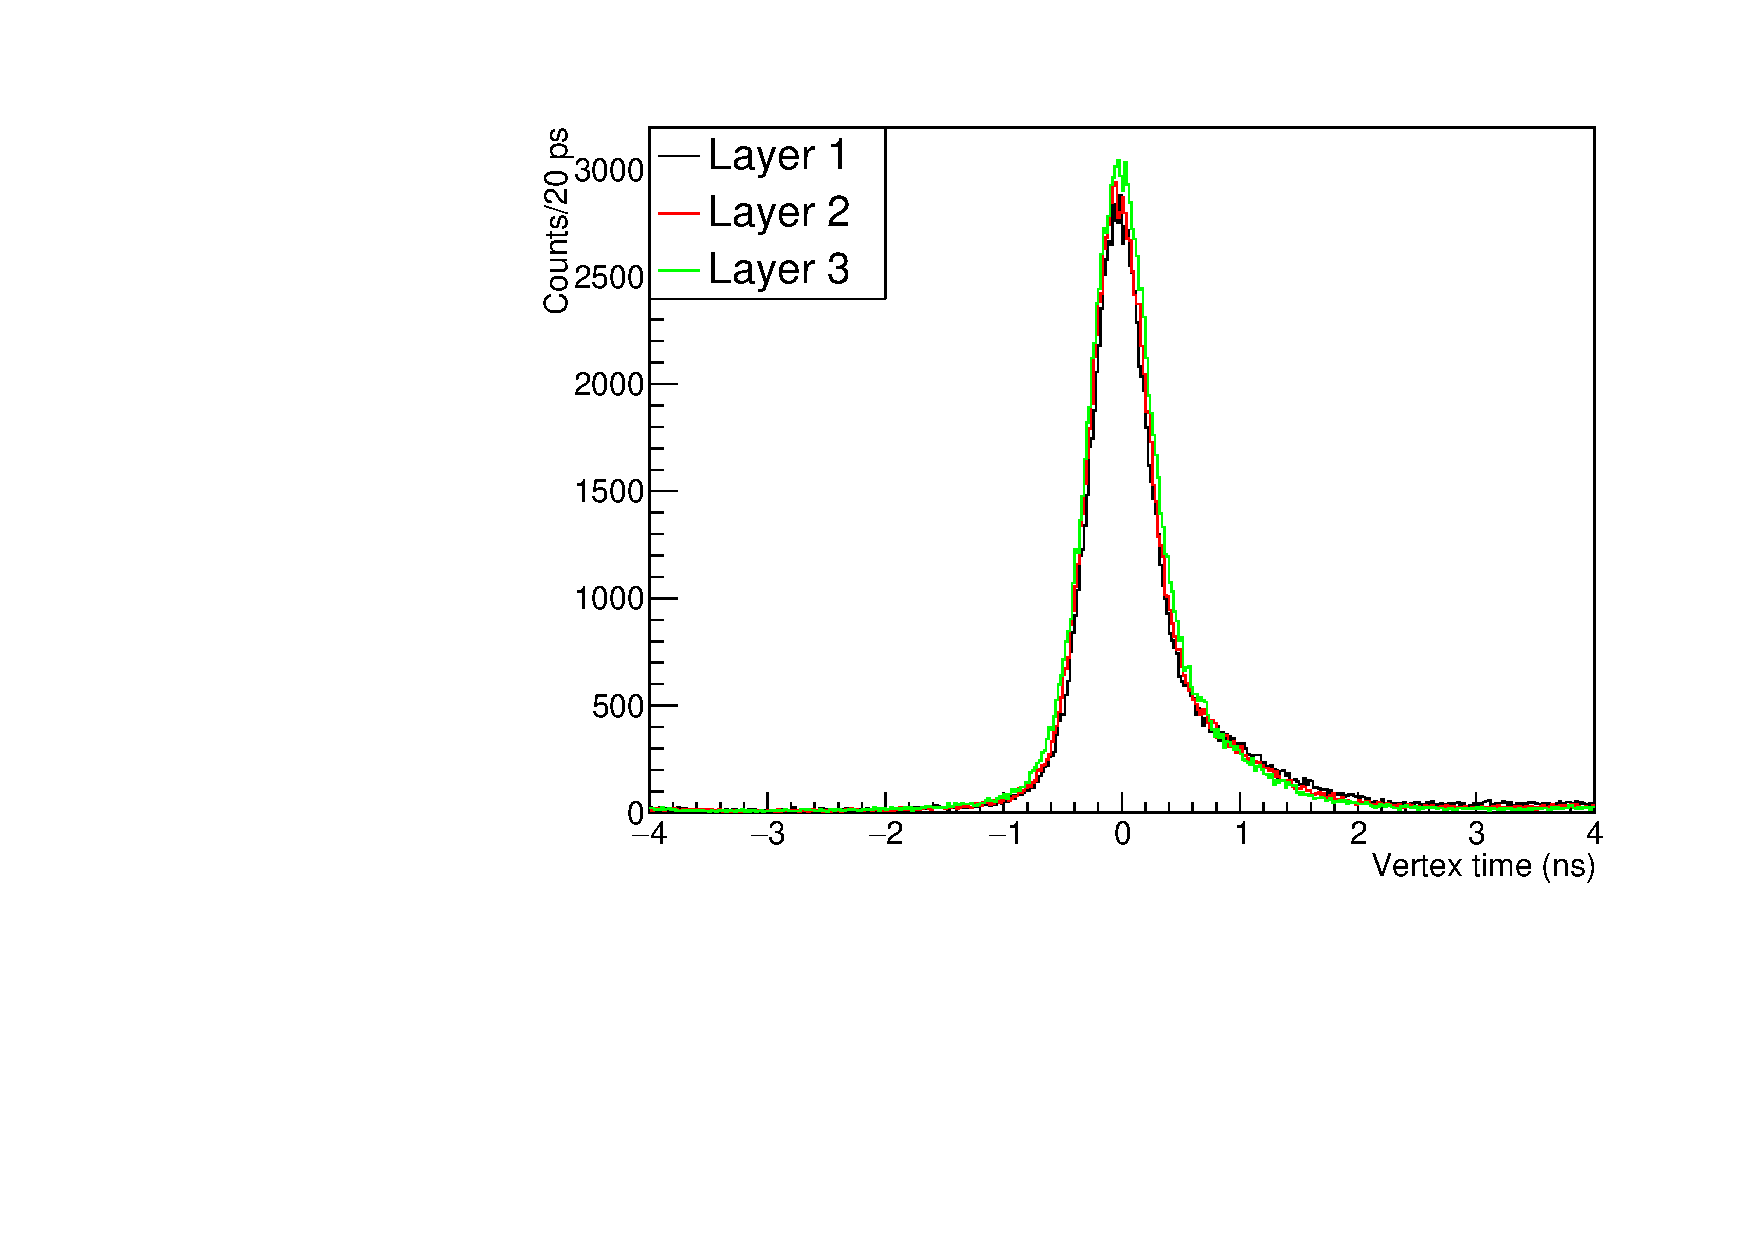
\includegraphics[width=0.45\textwidth]{Figure/canVTPlot.pdf}
\caption {Difference between the vertex time computed combining CND and CVT information and the start time computed by the FTOF, for negative tracks, for the three layers of the CND, integrated over all paddles. }
\label{fig_performance_deltat_layers}
\end{center}
\end{figure}

\begin{figure}[htb]  
\begin{center}
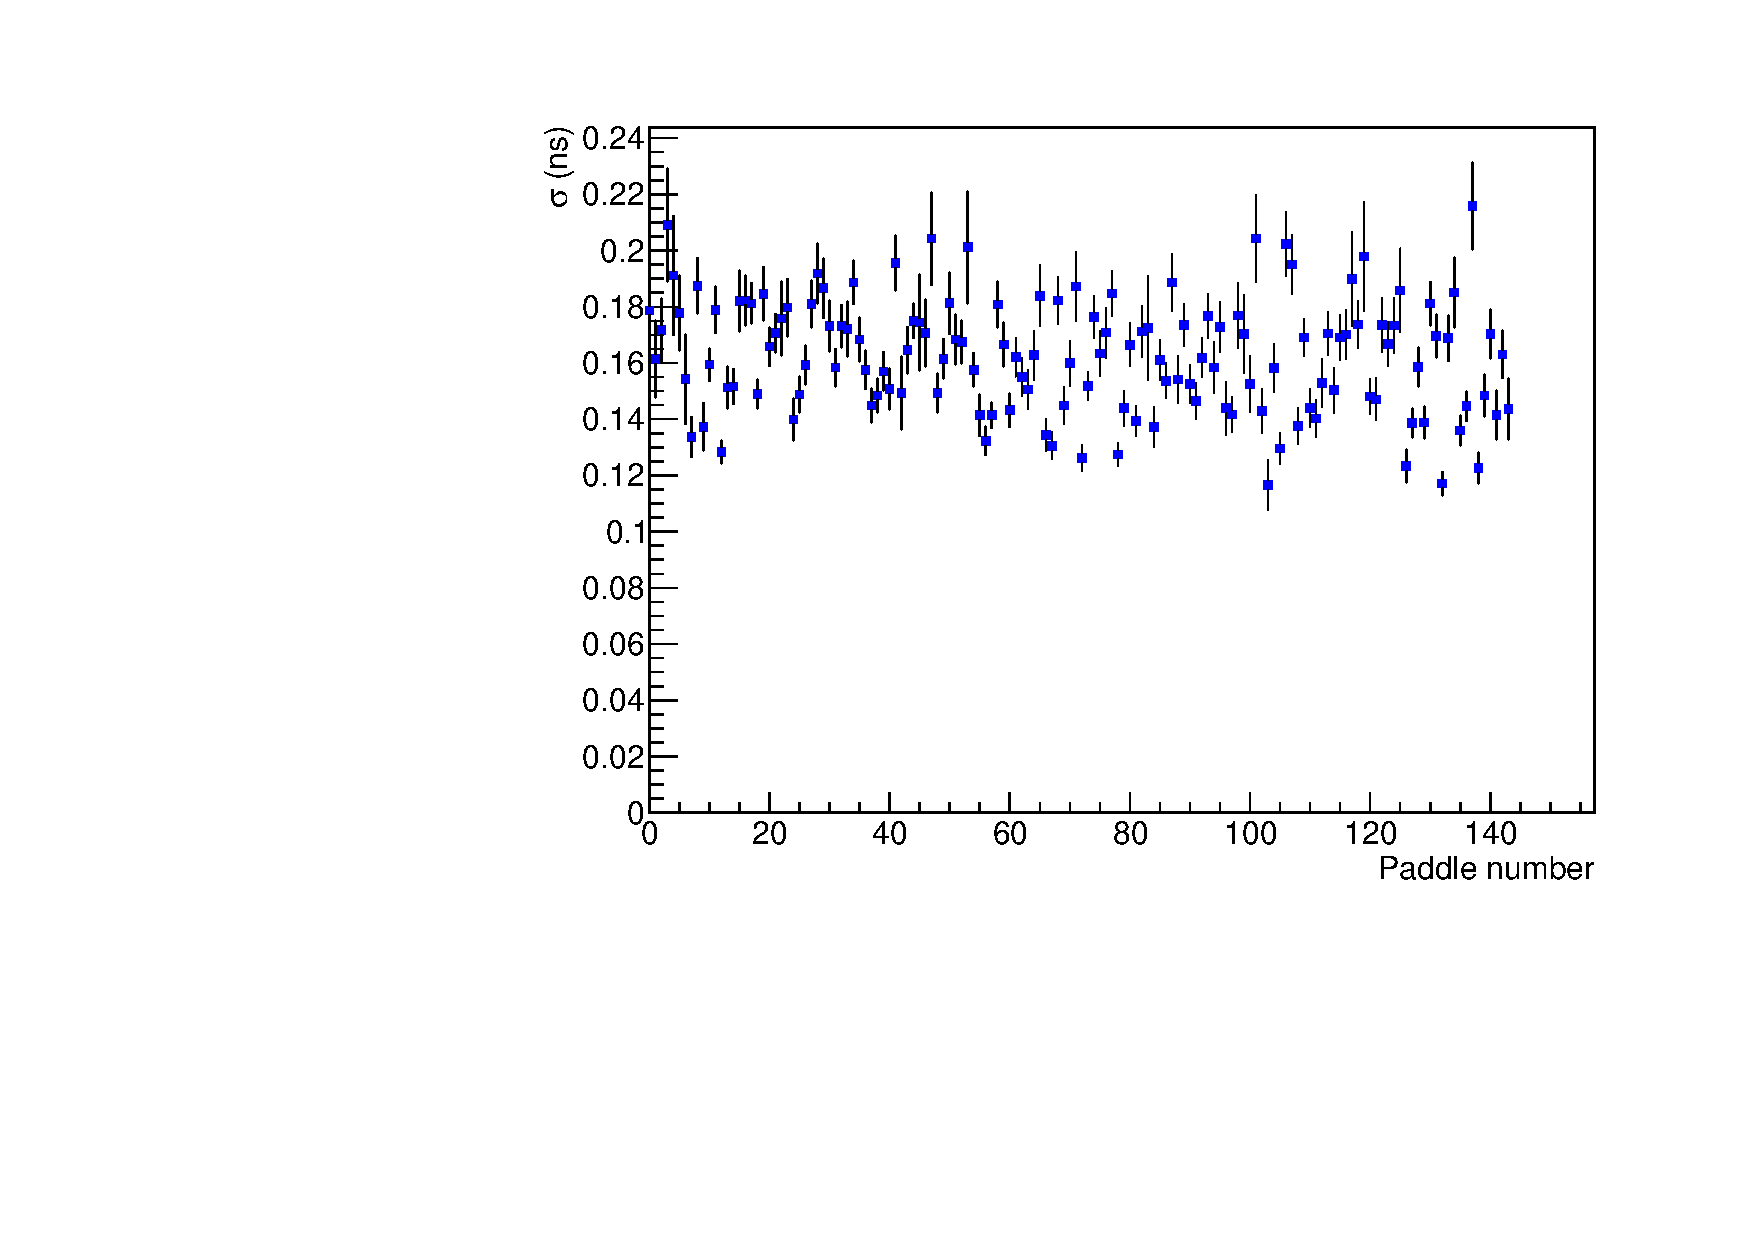
\includegraphics[width=0.45\textwidth]{Figure/VTsigma.pdf}
\caption {Timing resolution for each PMT of the CND, convoluted with CVT resolution.}
\label{fig_performance_vt_sigma_allpaddles}
\end{center}
\end{figure}

The position reconstruction performances of the CND can be checked in Fig.~\ref{fig_performance_deltaz}, which displays the difference between the $z$ coordinate computed by the CND and by the CVT, for negative tracks, and for the three layers of the CND, integrated over all paddles. Its Gaussian width is around 3 cm, corresponding roughly to $4^{\circ}$ in polar-angle resolution. This corresponds to the convolution of the angular resolutions of CND and CVT. 

\begin{figure}[htb]  
\begin{center}
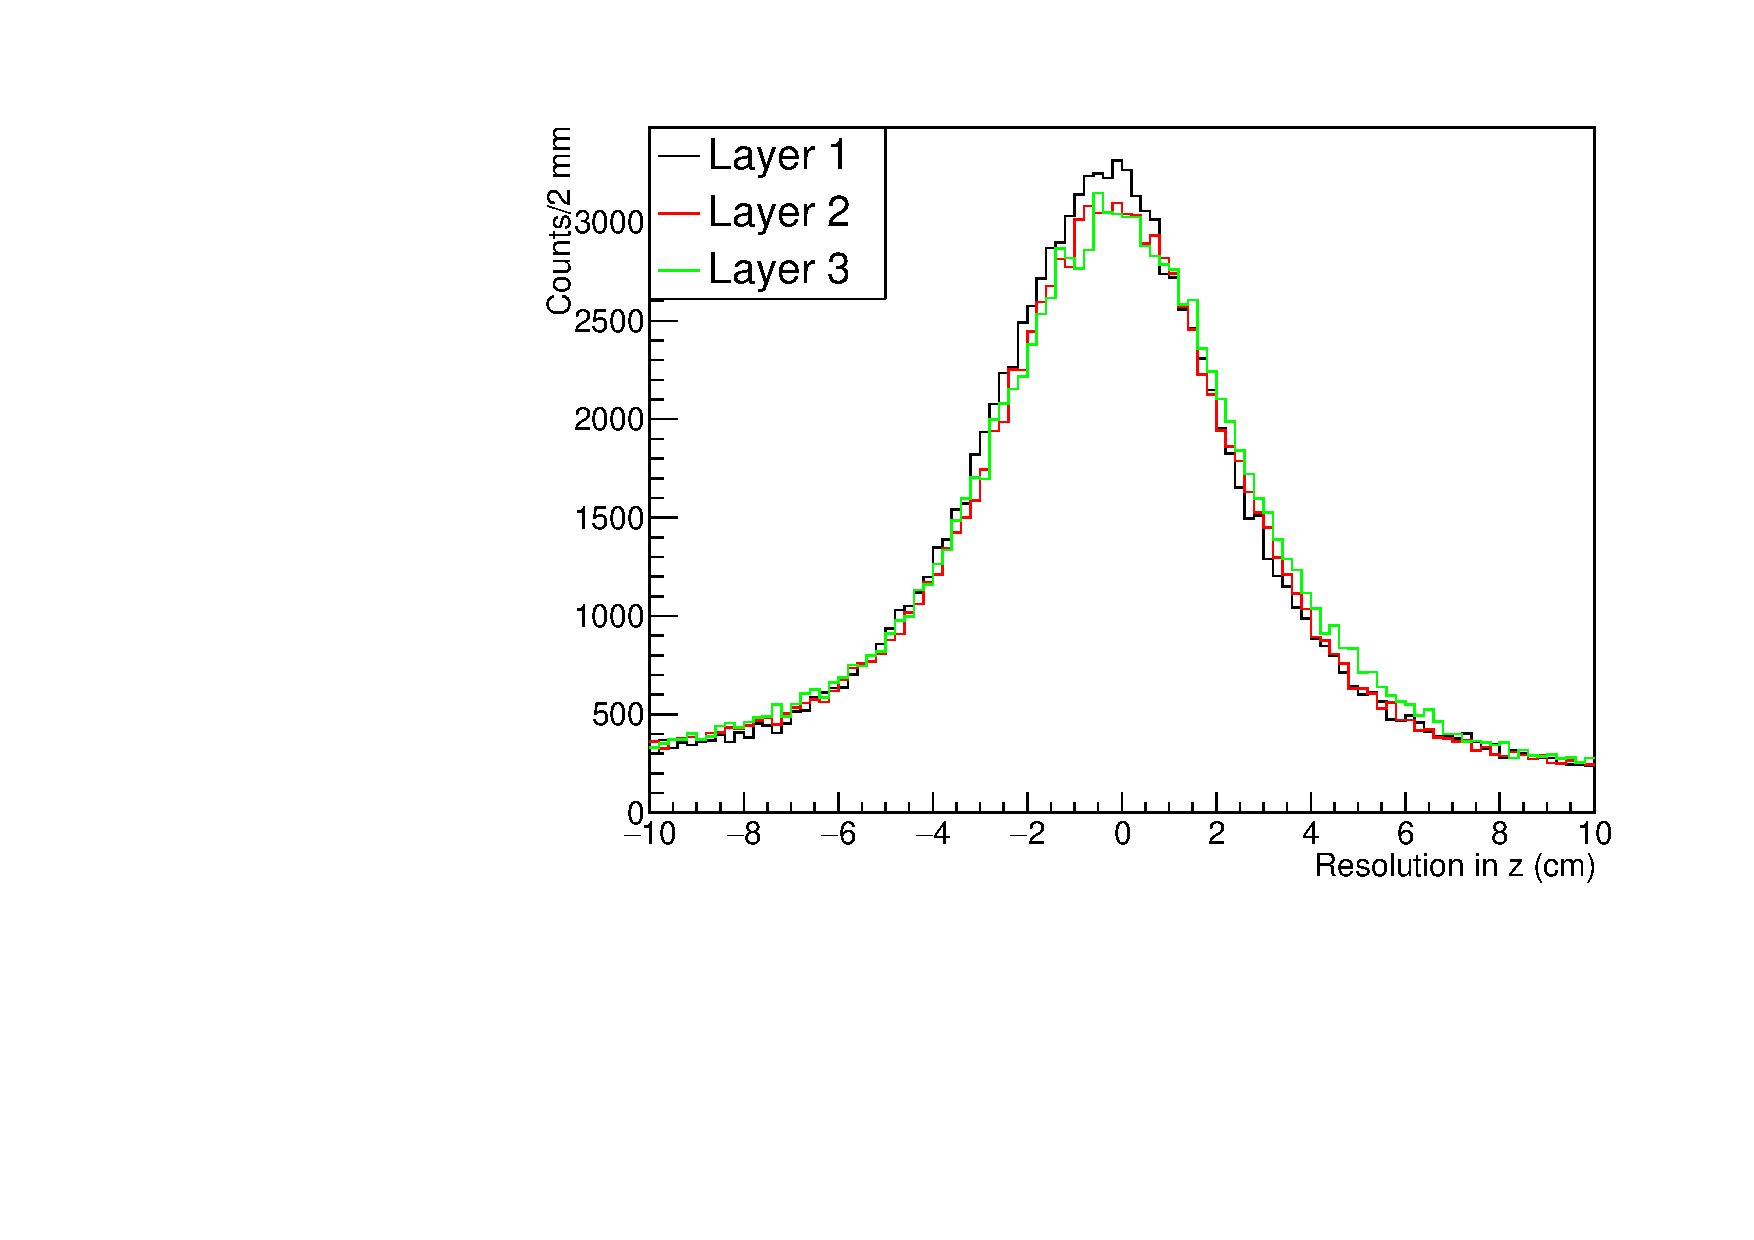
\includegraphics[width=0.45\textwidth]{Figure/canZ.pdf}
\caption {Difference between the $z$ computed by the CND and the one provided by the CVT, for negative tracks, for the three layers of the CND, integrated over all paddles. }
\label{fig_performance_deltaz}
\end{center}
\end{figure}

Figure~\ref{fig_performance_edep} shows the energy deposit divided by path length, for selected MIPs. It peaks at around the expected value of 1.956 MeV/cm.

\begin{figure}[htb]  
\begin{center}
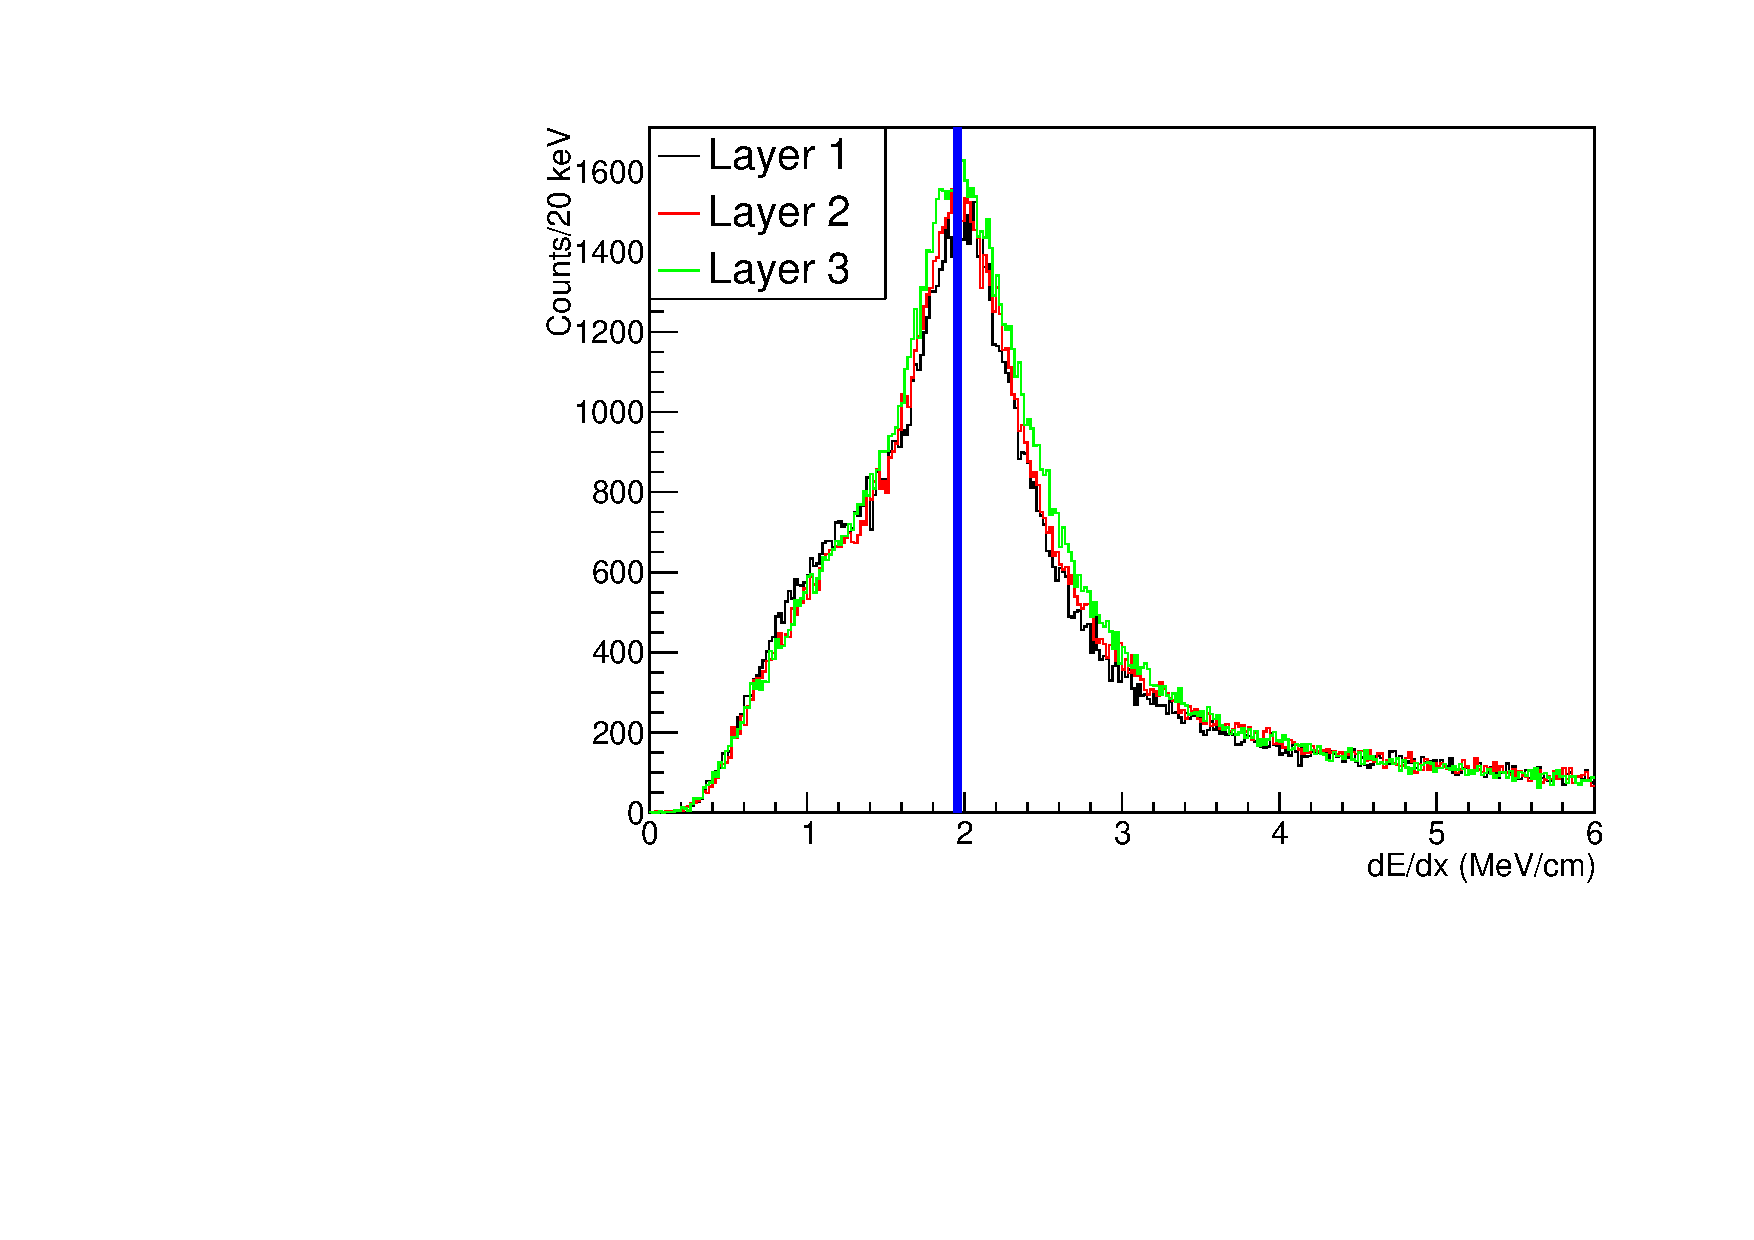
\includegraphics[width=0.45\textwidth]{Figure/canENE.pdf}
\caption {$dE/dx$ for MIPs in the three layers of the CND, integrated over all sectors. The blue line indicates the nominal value for the expected energy deposit of a MIP in a centimeter of plastic scintillator.}
\label{fig_performance_edep}
\end{center}
\end{figure}

NEUTRON EFFICIENCY FIGURES ARE NOT READY YET, WE'RE WAITING FOR RGK DATA TO BE COOKED.
